% !TeX root = RJwrapper.tex
\title{spinifex: A Package for Manual Control of Dynamic Linear Projections of
Multivariate Data}
\author{by Nicholas Spyrison, Dianne Cook}

\maketitle

\abstract{%
The set of dynamic linear projections of multivariate data collectively
known as \textbf{tours} provides an important tool for extending the
dimensionality of visuals. The R package \textbf{tourr} offers a variety
of path generators and geometric displays for conducting tours. This
paper discusses an extension package, \textbf{spinifex}, that adds
support for the path generation of manual tours and extends the display
of tours to use with the animation packages, \textbf{plotly} and
\textbf{gganimate}. Manual tours are used to explore the sensitivity of
structure as the contributions of a manipulation variable are changed. A
recent paper (Wang et al.
\protect\hyperlink{ref-wang_mapping_2018}{2018}) visualized the
sensitivity of the hadronic experiments to nucleon structure.
Sensitivity was characterized in non-linear 3D embeddings of the first
10 principal components. This research applies manual tours to this data
showing that manual tours resolve information about the structure of
cluster distribution by bringing to light information that is orthogonal
to static viewing planes.
}


\bibliography{spinifex_paper}

\hypertarget{introduction}{%
\section{Introduction}\label{introduction}}

A tour is a multivariate data analysis technique in which a sequence of
linear (orthogonal) projections are viewed as an animation while the
orientation of the projection basis is rotated across time. Each frame
of the sequence corresponds to a small change in the projection for a
smooth transition that preserves continuity. Tours are a crucial tool
extending the dimensionality of visualization which is increasingly
important as datasets and models exist in increasing cardinality. The
package \CRANpkg{tourr} (Wickham et al.
\protect\hyperlink{ref-wickham_tourr_2011}{2011}) builds a platform for
generating tour paths and applying to a wide number of display
geometrics in \textbf{base} graphics.

While there are numerous methods that generate tour paths, this research
focuses on the manual tour. The manual tour was described in Cook and
Buja (\protect\hyperlink{ref-cook_manual_1997}{1997}) and allows a user
to control the projection coefficients of a selected variable in a 2D
projection. The manipulation of these coefficients allows the analyst to
explore how sensitive the projection structure is to these
manipulations. As manual tours operate on only one variable at a time,
they particularly useful once a feature of interest has been identified.
One way to identify ``interesting'' features is with the use of a guided
tour (Hurley and Buja
\protect\hyperlink{ref-hurley_analyzing_1990}{1990}). Guided tours
select a very specific path, that which approaches a projection that
optimizes an objective-function, similar to simulated annealing
(Kirkpatrick, Gelatt, and Vecchi
\protect\hyperlink{ref-kirkpatrick_optimization_1983}{1983}). The direct
optimization of a function allows guided tours to rapidly identify
interesting projection features given the relatively large
parameter-space. After a projection of interest is identified an analyst
can then use the ``finer brush'' of the manual tour, by controlling the
contributions of individual variables to explore the sensitivity they
have to the projection structure.

This paper offers an implementation of manual tours with the package
\CRANpkg{spinifex}. This package also extends the graphics display of
\textbf{tourr} to the animation frameworks offered by \CRANpkg{plotly}
(Sievert \protect\hyperlink{ref-sievert_plotly_2018}{2018}) and
\CRANpkg{gganimate} (Pedersen and Robinson
\protect\hyperlink{ref-pedersen_gganimate:_2019}{2019}). The algorithm
used to perform a radial manual tour is demonstrated on a toy data set.
Followed by an application and discussion of the radial manual tour on
an aggregation of high energy physics experiments in a large
multivariate space.

The paper is organized as follows. Section \ref{sec:algorithm} explains
the algorithm using a toy dataset. Section \ref{sec:display} discusses
the display of the animation after the path has been generated. Section
\ref{sec:usage} explains the package functionality and code usage
following the order applied in the algorithm. Section
\ref{sec:application} illustrates how this can be used for sensitivity
analysis applied to contemporary high energy physics. The last section,
\ref{sec:discussion} summarizes the work and discusses future research.

\hypertarget{sec:algorithm}{%
\section{Algorithm}\label{sec:algorithm}}

The section below describes the algorithm for performing a 2D radial
manual tour:

\begin{enumerate}
\def\labelenumi{\arabic{enumi}.}
\tightlist
\item
  Provided with a 2D projection, choose a variable to manipulate. This
  is called the ``manip var''.
\item
  Create a 3D manipulation space, where the manip variable has the full
  contribution.
\item
  Generate a rotation sequence which increases the norm of the
  coefficient to 1 and zeros it.
\end{enumerate}

The steps are described in more detail below with descriptions,
equations, and figures are given inline. Function names are mentioned,
but code usage is discussed in more detail in section \ref{sec:usage}.

\hypertarget{notation}{%
\subsection{Notation}\label{notation}}

This section describes the notation used in the algorithm for a 2D
radial manual tour.

\begin{itemize}
  \item $\textbf{X}$, the data, an $n \times p$ numeric matrix to be embedded in two dimensions.
  \item $\textbf{B} = (B_1,~ B_2)$, any orthonormal projection basis set, $p \times 2$ matrix, describing the projection from $p$ to two dimensions
  \item $\textbf{e}$, a zero column vector of length $p$ with the $k-$th element set to one, where $k$ is the number of the variable to manipulate, the manip var.
  \item $\theta$, the angle of in-projection-plane rotation, for example, on the reference axes.
  \item $\phi$, the angle of out-of-projection-plane rotation, coming into the manipulation space.
\end{itemize}

The algorithm primarily operates on projection bases and utilizes the
data only when making a display. The projection space can be viewed at
any point in the process by pre-multiplying the data and plotting the
first two variables.

\hypertarget{toy-data-set}{%
\subsection{Toy data set}\label{toy-data-set}}

The flea data, originally from Lubischew
(\protect\hyperlink{ref-lubischew_use_1962}{1962}), made available in
\textbf{tourr} is used to illustrate the algorithm. The data contains 74
observations across 6 variables, which are physical measurements of the
flea beetles. Each observation belongs to one of three species.

The data is defined. A basis set (ideally orienting to an interesting
feature) must be provided as an initial orientation. One way to identify
a projection containing interesting features is to apply a guided tour.
In a guided tour, the projection sequence is selected by optimizing an
index function via hill-climbing on the projection space. In this case,
the holes index is selected and applied to standardized flea data. The
holes index is maximized when the projected observations are furthest
from the center. Figure \ref{fig:step0} shows a locally optimized
projection of the data. The left panel displays the reference axes of
the projection basis, a visual indication of the magnitude and direction
each variable contributed to the projection. The right panel shows the
data as projected through the basis set described by the reference axes
(left). Data points are colored and given shape according to the species
(while the guided tour was unsupervised with this information).

\begin{Schunk}
\begin{figure}

{\centering 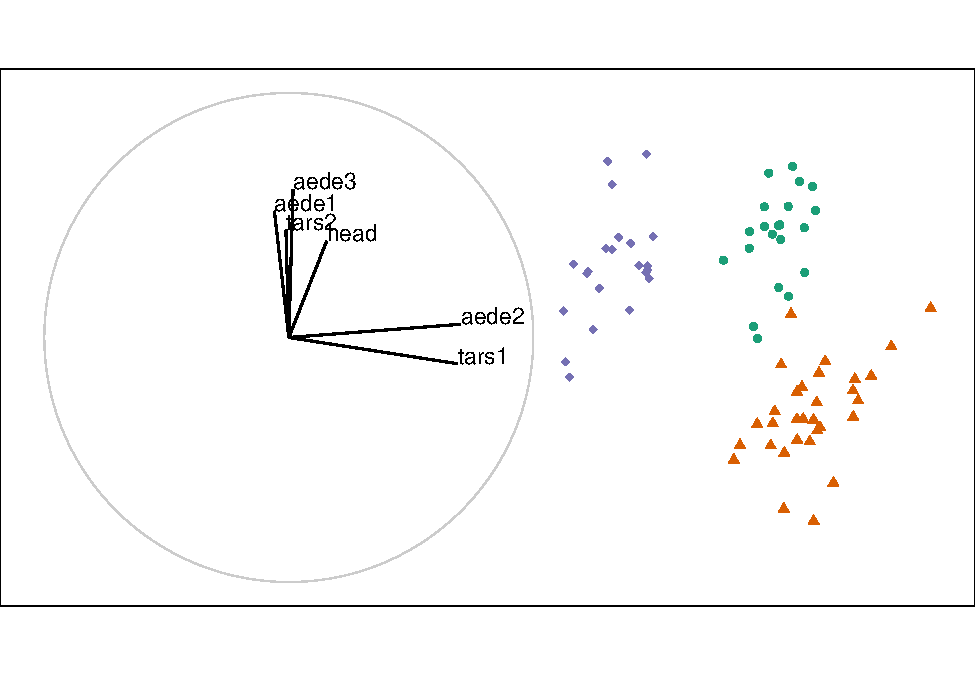
\includegraphics[width=0.7\linewidth]{spinifex_paper_files/figure-latex/step0-1} 

}

\caption[Basis reference axes (left) and projected data (right) of standardized flea data]{Basis reference axes (left) and projected data (right) of standardized flea data. Data points color and shape are mapped to beetle species. The basis was identified by a holes-index guided tour. The variables aede2 and tars1 contribute mostly orthogonal to the other variables.}\label{fig:step0}
\end{figure}
\end{Schunk}

Call \texttt{view\_basis()} on a basis to produce a \CRANpkg{ggplot2}
(Wickham \protect\hyperlink{ref-wickham_ggplot2:_2016}{2016}) graphic
similar to \textbackslash ref\{fig:step0). Projection space is always
available for display via the matrix multiplication
\(\textbf{X}_{[n,~p]} ~*~ \textbf{B}_{[p,~d]} ~=~ \textbf{P}_{[n,~d]}\).

\hypertarget{step-1-choose-variable-of-interest}{%
\subsection{Step 1) Choose variable of
interest}\label{step-1-choose-variable-of-interest}}

In figure \ref{fig:step0} the contributions of the variables tars1 and
aede2 are mostly orthogonal to the contributions of the other four
variables. These two variables explain the variation of the data
distinguishing the purple group from the rest of the sample. Select
aede2 as the manip var, the variable to be manipulated, as it has a
larger contribution to the projection. The question that will be
explored is how important the variable aede2 is to the separation of the
clusters.

\hypertarget{step-2-create-the-manip-space}{%
\subsection{Step 2) Create the manip
space}\label{step-2-create-the-manip-space}}

Initialize a zero vector \textbf{e} of length \emph{p}. Set the fifth
element to one, as aede2 is the fifth variable in the data, giving the
manip var a full contribution in this dimension. Use the Gram-Schmidt
process to orthonormalize the zero vector onto the basis yielding the 3D
manipulation space, \textbf{M}.

\begin{align*}
  \textbf{e}_k &\leftarrow 1 \\ 
  \textbf{e}   &\leftarrow \textbf{e} - \langle \textbf{e}, \textbf{B}_1 \rangle \textbf{B}_1 - \langle \textbf{e}, \textbf{B}_2 \rangle \textbf{B}_2 \\ 
  \textbf{M}_{[p,~3]} &= (\textbf{B}_1,\textbf{B}_2,\textbf{e})
\end{align*}

Adding this new dimension to our projection space allows for the
coefficients of the manip var to be changed via rotation about the
origin. For example, the ability to lift a piece of paper, rather than
being constrained to a 2D plane. Orthonormalizing rescales the new
vector while the projection down to 2D remains the original basis. Place
the plane horizontally, with the new dimension extending vertically,
with axes projecting back onto the reference axes. Figure
\ref{fig:step2} illustrates this 3D manipulation space with the manip
var highlighted (height of the other variables are not depicted.)

\begin{Schunk}
\begin{figure}

{\centering 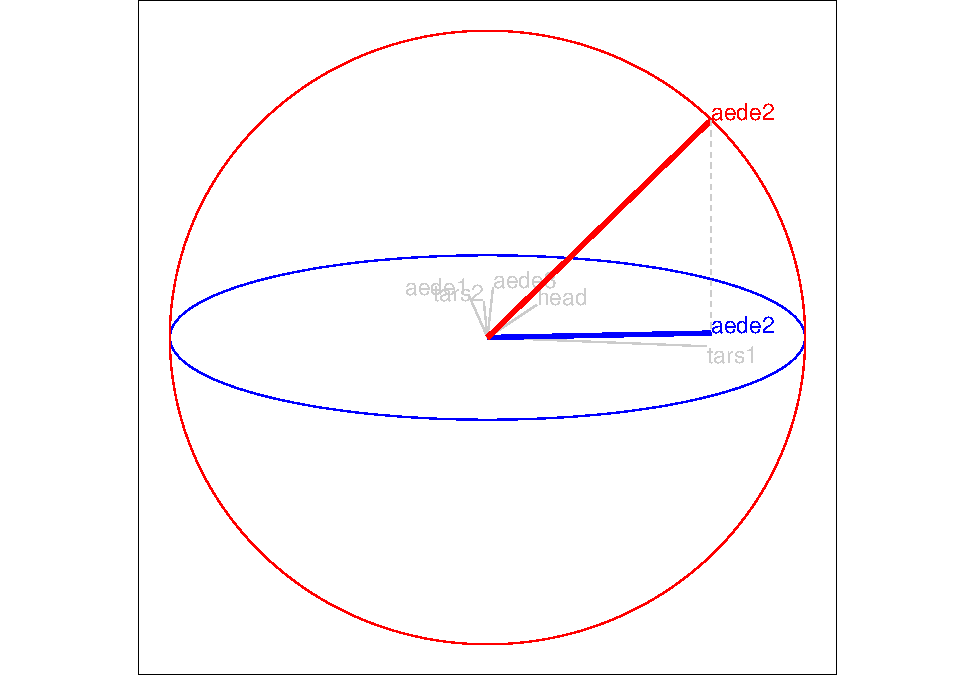
\includegraphics[width=0.7\linewidth]{spinifex_paper_files/figure-latex/step2-1} 

}

\caption[Manipulation space for controlling the contribution of aede2 of standardized flea data]{Manipulation space for controlling the contribution of aede2 of standardized flea data. Basis selected by a holes-index optimized guided tour lies on the horizontal projection plane, shown in blue. The manip var axis, in red, extends into the vertical manipulation space, allowing the coefficients of the manip var to be changed by rotation around the origin.}\label{fig:step2}
\end{figure}
\end{Schunk}

The representation in figure \ref{fig:step2} can be produced by calling
the function \texttt{view\_manip\_space()}.

\hypertarget{step-3-generate-rotation}{%
\subsection{Step 3) Generate rotation}\label{step-3-generate-rotation}}

Imagine holding the manip var, the red axis, one end fixed to the
origin. As it is controlled the manipulation space rotates about the
origin, the projection onto the horizontal projection plane
correspondingly moves. This is what happens in a manual tour. Generating
a sequence of values for the horizontal and vertical, angles produces a
path for the rotation of the manipulation space. This defines the
(orthonormally-constrained) rotation on the coefficients of the
variables.

For a radial tour fix the (horizontal) angle within the projection
plane, \(\theta\), and define a sequence for the (vertical) angle coming
out of the projection plane, \(\phi\), bringing the initial \(XY\)
contributions of the manip var to a maximum and then to zero before
returning to the initial position. Dynamic capture of user manipulation
is typically performed directly on the projection plane (without
depiction of the manipulation space.)

Post-multiply the manipulation space by the pre-defined rotation matrix
producing \textbf{RM}, the rotated manip space. This is one frame of
basis values, repeat this process for each value in the sequences of
\(\theta\) and \(\phi\) for the complete animation.

Let:

\begin{itemize}
  \item[$c_\theta$] be the cosine of $\theta$
  \item[$c_\phi$]   be the cosine of $\phi$
  \item[$s_\theta$] be the sine of   $\theta$
  \item[$s_\phi$]   be the sine of   $\phi$
\end{itemize}

\textbf{For each value of } \(i\) \textbf{:}

\begin{align*}
  \textbf{RM}_{[p,~3,~i]}
  &= \textbf{M}_{[p,~3]} ~*~ \textbf{R}_{[3,~3,~i]} \\
  &= \textbf{M}_{[p,~3]}
    ~*~
  \begin{bmatrix}
    c_\theta^2 c_\phi s_\theta^2 &
    -c_\theta s_\theta (1 - c_\phi) &
    -c_\theta s_\phi \\
    -c_\theta s_\theta (1 - c_\phi) &
    s_\theta^2 c_\phi + c_\theta^2 &
    -s_\theta s_\phi \\
    c_\theta s_\phi &
    s_\theta s_\phi &
    c_\phi
  \end{bmatrix}_{[3,~3,~i]}
\end{align*}

A note on application: \(\phi\) is the angle relative to the initial
value of \(\phi\), we find the transformation \(\phi_i\) - \(\phi_1\)
useful to think about \(\phi\) relative to the basis plane.
Additionally, the value of \(\phi\) may be out of phase by a factor of
pi. If the manip variable doesn't move as expected these are the first
places to check.

Figure \ref{fig:step3} illustrates a sequence with 15 projected bases,
showing the reference axes on top the corresponding projected data
points on the below. As a result, we can see that changes in the manip
var controlled the distance between the purple cluster and the remaining
sample, aede2 is crucial in distinguishing this species. Tours are
typically viewed as an animation such a dynamic version of this tour can
be viewed online at
\url{https://nspyrison.netlify.com/thesis/flea_manualtour_mvar5/}. The
page may take a moment to load.

\begin{Schunk}
\begin{figure}

{\centering 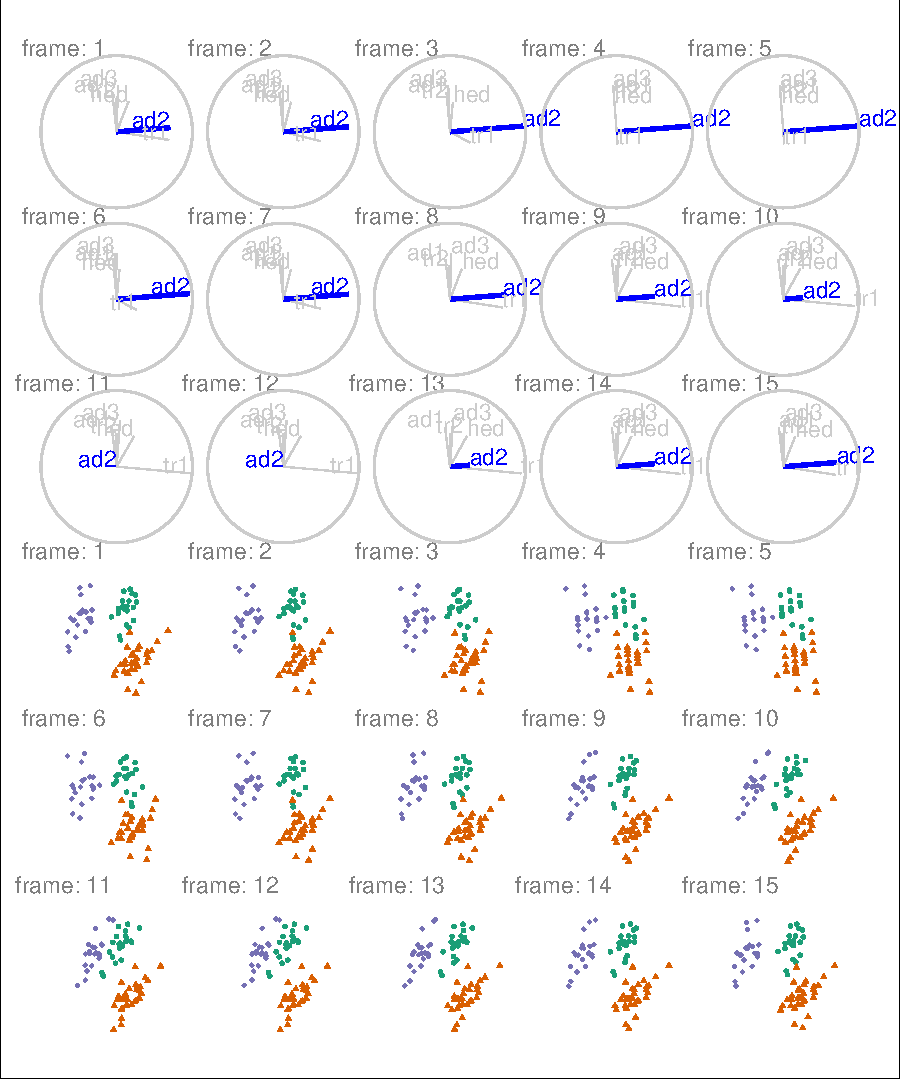
\includegraphics[width=6in,height=7.2in]{spinifex_paper_files/figure-latex/step3-1} 

}

\caption[Radial manual tour manipulating aede2 of standardized flea data]{Radial manual tour manipulating aede2 of standardized flea data.  The contributions increase from its initial contribution to a full contribution to the projection before decreasing to zero and then returning to its initial value. The change in the projected data shows that aede2 is important for distinguishing the purple species. An animated version can be viewed at  https://nspyrison.netlify.com/thesis/flea\_manualtour\_mvar5/.}\label{fig:step3}
\end{figure}
\end{Schunk}

Animations can be produced using the function
\texttt{play\_manual\_tour()}. This function defaults to an HTML5 widget
produced from \textbf{plotly}. The \texttt{render\_type} argument can be
changed to \texttt{render\_gganimate} for exporting to GIF or MP4 files.

\hypertarget{sec:display}{%
\section{Data in projection-space}\label{sec:display}}

In an appeal to performance, the above operations are performed on the
bases without the use of the larger datasets. After the bases are
brought into the projection-space, however, it is helpful to observe
them with data in the same space. Pre-multiply the data by basis frame
bringing the data into the projection space.

\begin{align*}
  \textbf{P}_{[n,~3]} &= \textbf{X}_{[n,~p]} ~*~ \textbf{RM}_{[p,~3]}
\end{align*}

For a 2D scatterplot, plot the first two variables from each frame
statically as in the previous figure, or in sequence, producing an
animated scatterplot. The remaining variable is sometimes linked to a
data point aesthetic (such as size or color) to produce depth cues used
in conjunction with the \(XY\) scatterplot.

\hypertarget{sec:usage}{%
\section{Package structure and functionality}\label{sec:usage}}

This section discusses the functions and code usage of the package
before delving into a domain-specific application of the manual tour.

\hypertarget{installation}{%
\subsection{Installation}\label{installation}}

\begin{Schunk}
\begin{Sinput}
# remotes::install_github("nspyrison/spinifex") # Development version
install.package("spinifex")
library("spinifex")

# Also see the vignette: 
vignette("spinifex_vignette")
\end{Sinput}
\end{Schunk}

\hypertarget{primary-package-functions}{%
\subsection{Primary package functions}\label{primary-package-functions}}

The primary functions that will aid users in performing their own manual
tours are broken into the following groupings: tour preparation, tour
animation, and utility.

\begin{Schunk}
\begin{table}[t]

\caption{\label{tab:functionsTable}Primary functions}
\centering
\begin{tabular}{lll}
\toprule
Class & Function & Description\\
\midrule
tour preparation & view\_basis & displays the reference frame of the basis\\
tour preparation & view\_manip\_space & displays the manipulation space\\
tour animation & play\_tour\_path & animates given tour path\\
tour animation & play\_manual\_tour & animates the manual tour algorithm\\
utility & render\_gganimate & uses gganimate to render the animation\\
\addlinespace
utility & render\_plotly & uses plotly to render the animation\\
\bottomrule
\end{tabular}
\end{table}

\end{Schunk}

In the following section describes and shows usage of the tour related
functions in parallel with the algorithm. The utility functions are
called by the tour animation functions, passed to the arguments
\texttt{render\_type}. Usage is demonstrated below and in the example
documentation.

\hypertarget{algorithm-code}{%
\subsection{Algorithm code}\label{algorithm-code}}

We'll start by initializing values including a standardized data set
(numeric columns only), a starting basis, a categorical variable for
point aesthetics, and a manip var. To get bearings on the projection,
start by observing the reference axes of the basis with
\texttt{view\_basis()}.

\begin{Schunk}
\begin{Sinput}
f_data  <- tourr::rescale(flea[, 1:6])                    ## standardize data
f_path  <- save_history(f_data, guided_tour(holes()))     ## produce guided tour
f_basis <- matrix(f_path[,, max(dim(f_path)[3])], ncol=2) ## end of guided tour
f_cat   <- factor(flea$species)                           ## categorical var

view_basis(basis = f_basis, 
           data = f_data,
           labels = colnames(f_data))
\end{Sinput}
\end{Schunk}

After becoming familiar with this space, select a manip var, the
variable to change the contributions of. Use
\texttt{view\_manip\_space()} View the new space with a dimension
orthogonal to the projection plane where the manip var has a full
contribution. This illustrates how the manip var is manipulated in a
high space not depicted in the manual tour.

\begin{Schunk}
\begin{Sinput}
f_mvar  <- 5  ## manip var numebr

view_manip_space(basis = f_basis, 
                 manip_var = f_mvar, 
                 labels = colnames(f_data))
\end{Sinput}
\end{Schunk}

Now we are ready to perform a manual tour on the selected variable. Use
\texttt{play\_manual\_tour()} to perform the algorithm as discussed
above, in section \ref{sec:algorithm}. The argument
\texttt{render\_type} can be changed to \texttt{render\_gganimate} for a
respective animation.

\begin{Schunk}
\begin{Sinput}
angle_speed <- .26

play_manual_tour(data = f_data,
                 basis = f_basis, 
                 manip_var = f_mvar, 
                 angle = angle_speed,
                 col = f_cat,
                 pch = f_cat)
\end{Sinput}
\end{Schunk}

Aside from the code used in the algorithm section a previously generated
tour path can also be animated via \texttt{play\_tour\_path()}. Utility
functions can also be passed into arguments: for example animation
format can be changed by setting
\texttt{render\_type\ =\ render\_gganimate}. View the guided tour path
as a gganimate function:

\begin{Schunk}
\begin{Sinput}
play_tour_path(tour_path = f_path,
               data = f_data,
               render_type = render_gganimate, 
               angle = angle_speed
)
\end{Sinput}
\end{Schunk}

\hypertarget{rendering-and-sharing}{%
\subsection{Rendering and sharing}\label{rendering-and-sharing}}

The \textbf{tourr} package utilizes \textbf{base} graphics for the
display of tours. \textbf{spinifex} allows tours to be used in rendered
in \textbf{plotly} as an HTML5 object or \textbf{gganimate} as GIF or
MP4 files. Both of which build off \textbf{ggplot2} objects in internal
functions. Sharing of animations is not trivial especially in print and
static file formats such as PDF. Even with the use of computers and
dynamic file formats capturing the correct resolution, aspect, and
display is challenging and many formats quickly bloat file sizes. Keep
in mind hosting options and exporting functions from \textbf{plotly},
\textbf{gganimate} and \textbf{tourr}.

\hypertarget{storage}{%
\subsection{Storage}\label{storage}}

Storing each data point for every frame of the animation is redundant.
Just as operations are performed on the bases, so too should tour paths
be stored as bases and a single instance of the data. Consider a radial
manual tour, we can store the salient features in 3 bases, where
\(\phi\) is at its starting, minimum, and maximum values. The frames in
between can be interpolated by supplying angular speed. With the use of
the \texttt{tourr::save\_history()} function, the target bases can be
saved. From there geodesic interpolation can be used to populate the
intermittent frames. This type of interpolation should not be used on
manual tours, which have already been initialized into a 3D manipulation
space where direct linear interpolation is appropriate.

\hypertarget{sec:application}{%
\section{Application}\label{sec:application}}

In a recent paper, Wang et al.
(\protect\hyperlink{ref-wang_mapping_2018}{2018}), the authors aggregate
and visualize the sensitivity of hadronic experiments to nucleon
structure. The authors introduce a new tool, PDFSense, to aid in the
visualization of Parton distribution functions (PDF). The
parameter-space of these experiments lies in 56 dimensions,
\(\delta \in \mathbb{R}^{56}\), and are visualized as 3D subspaces of
the 10 first principal components in linear (PCA) and non-linear (t-SNE)
embeddings.

Using the same data, another study, Cook, Laa, and Valencia
(\protect\hyperlink{ref-cook_dynamical_2018}{2018}), applies grand tours
(Asimov \protect\hyperlink{ref-asimov_grand_1985}{1985}) to the same
subspaces. Grand tours are dynamic subspace projections of high
dimensional where frames and selected at random and linked with
geodesically interpolation of the intermediate frames. Grand tours are
able to better resolve the distribution shape of clusters, intra-cluster
detail, and better outlier detection than the use of PDFSense \& TFEP
(TensorFlow embedded projections). Before applying manual tours let's
discuss the structure of the data.

The data has a hierarchical structure with top-level clusters; DIS, VBP,
and jet. Each cluster is a particular class of experiments, each with
many experimental datasets which, in turn, have many observations. In
the consideration of data density, we conduct manual tours on subsets of
the DIS and jet clusters. This explores the sensitivity of the structure
to each of the variables in turn and we present the subjectively best
and worst variable to manipulate for identifying dimensionality of the
clusters and describing the span of the clusters.

\hypertarget{jet-cluster}{%
\subsection{Jet cluster}\label{jet-cluster}}

The jet cluster resides in a smaller dimensionality than the full set of
experiments with four principal components explaining 95\% of the
variation in the cluster (Cook, Laa, and Valencia
\protect\hyperlink{ref-cook_dynamical_2018}{2018}). The data within this
4D embedding is subset down to ATLAS7old and ATLAS7new to focus in on
two groups with a reasonable number of observations that occupy
different parts of the subspace. Radial manual tours controlling
contributions from PC4 and PC3 are shown in figure
\ref{fig:JetClusterGood} and figure \ref{fig:JetClusterBad}
respectively. These components are selected to contrast the difference
of information conveyed by touring different variables. Links to dynamic
HTML5 animations controlling each of the four variables are also
provided.

When manipulating PC4, there is a clear difference in the parameter
space spanned by the experiment types ATLAS7new and ATLAS7old. Yet, when
PC3 is manipulated there is no indication that the different experiments
probe different parameter space. Performing a radial manual tour on PC4
is more insightful than for PC3.

Radial manual tours manipulating each of the principal components in the
jet cluster can be viewed by following the links:
\href{https://nspyrison.netlify.com/thesis/jetcluster_manualtour_pc1/}{PC1},
\href{https://nspyrison.netlify.com/thesis/jetcluster_manualtour_pc2/}{PC2},
\href{https://nspyrison.netlify.com/thesis/jetcluster_manualtour_pc3/}{PC3},
and
\href{https://nspyrison.netlify.com/thesis/jetcluster_manualtour_pc4/}{PC4}.

\begin{Schunk}
\begin{figure}

{\centering 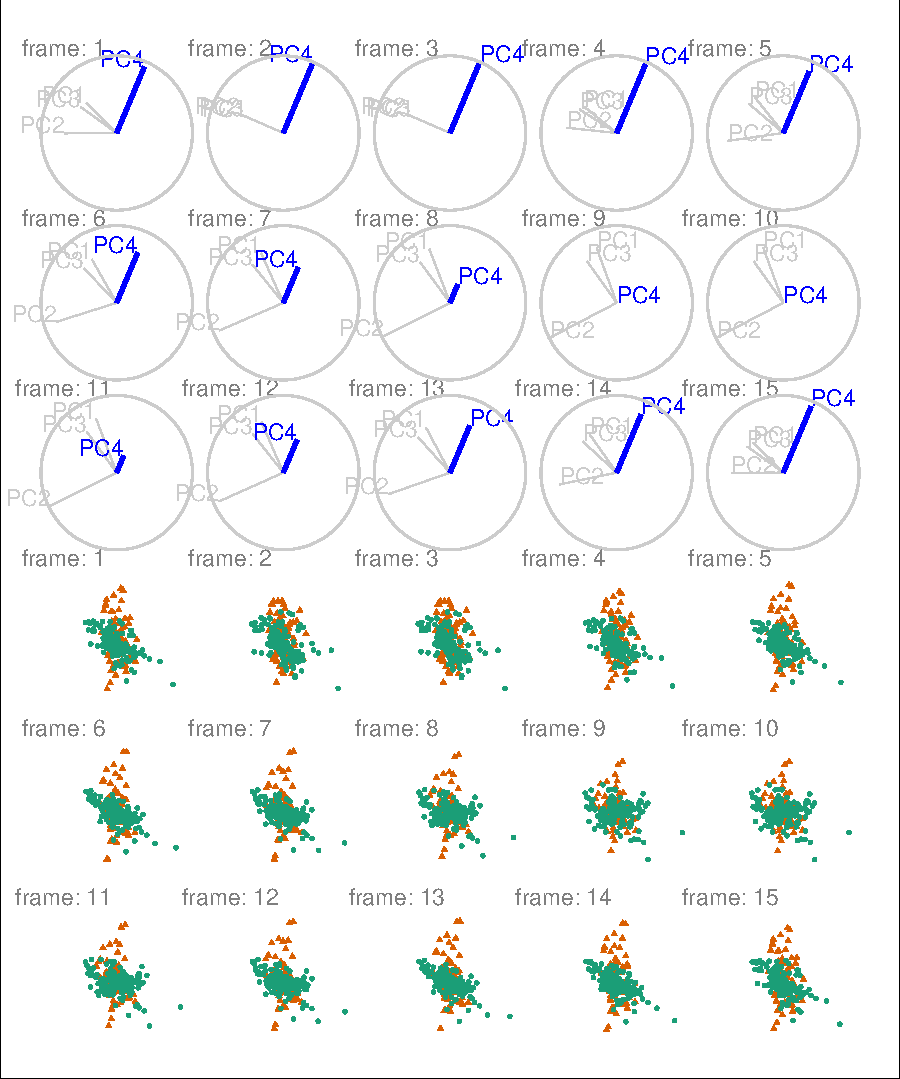
\includegraphics[width=6in,height=7.2in]{spinifex_paper_files/figure-latex/JetClusterGood-1} 

}

\caption[A radial manual tour of PC4 within the jet cluster]{A radial manual tour of PC4 within the jet cluster. Colored by experiment type: ATLAS7new in green and ATLAS7old in orange. When PC4 fully/negligibly contributes to the projection ATLAS7new (green) spans the same space as the orange points. During the intermediate frames, the ATLAS7new is compressed in the direction radial to PC4. A dynamic version can be viewed at https://nspyrison.netlify.com/thesis/jetcluster\_manualtour\_pc4/.}\label{fig:JetClusterGood}
\end{figure}
\end{Schunk}

\begin{Schunk}
\begin{figure}

{\centering 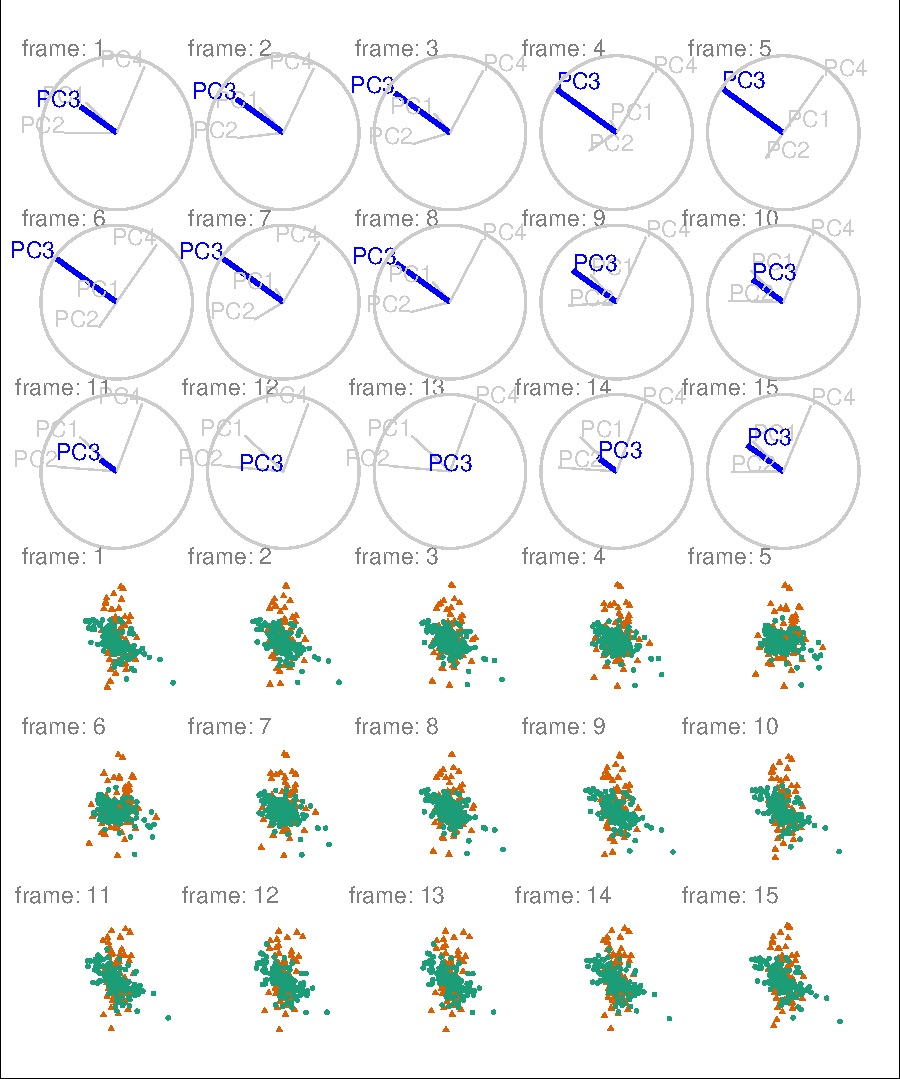
\includegraphics[width=6in,height=7.2in]{spinifex_paper_files/figure-latex/JetClusterBad-1} 

}

\caption[A radial manual tour of PC4 within the jet cluster]{A radial manual tour of PC4 within the jet cluster. Colored by experiment type: ATLAS7new in green and ATLAS7old in orange. Data from ATLAS7new (green) spans mostly the same space as ALTLAS7old (orange) with no evident difference in cluster structure across varying contributions of PC3. A dynamic version can be viewed at https://nspyrison.netlify.com/thesis/jetcluster\_manualtour\_pc3/.}\label{fig:JetClusterBad}
\end{figure}
\end{Schunk}

\hypertarget{dis-cluster}{%
\subsection{DIS cluster}\label{dis-cluster}}

A different space is used to explore the DIS cluster; specifically the
first six principal components, which explains 48\% of the variation
contained within the aggregated data (Cook, Laa, and Valencia
\protect\hyperlink{ref-cook_dynamical_2018}{2018}). Radial manual tours
are performed on PC6 and PC2 in figure \ref{fig:DISclusterGood} and
figure \ref{fig:DISclusterBad} respectively.

The selection of the manip variable is important as the manipulation
spaces convey substantially different information. The manual tour of
PC6 offers information about the dimensionality, shape, and orientations
of the different experiment classes. Whereas manipulating the
contributions of PC2 only shows a subset of the dimensionality and shape
information. Manipulating the contributions of PC6 turned out to be much
more insightful than that of PC2. This result might seem
counter-intuitive at first as PC2 should explain much more of the
variation in the data. However, features and structure in the data
regularly reside in finer detail that can be lost when looking only at
static projections.

DIS cluster manual tours manipulating each of the principal components
can be viewed from the links:
\href{https://nspyrison.netlify.com/thesis/discluster_manualtour_pc1/}{PC1},
\href{https://nspyrison.netlify.com/thesis/discluster_manualtour_pc2/}{PC2},
\href{https://nspyrison.netlify.com/thesis/discluster_manualtour_pc3/}{PC3},
\href{https://nspyrison.netlify.com/thesis/discluster_manualtour_pc4/}{PC4},
\href{https://nspyrison.netlify.com/thesis/discluster_manualtour_pc5/}{PC5},
and
\href{https://nspyrison.netlify.com/thesis/discluster_manualtour_pc6/}{PC6}.

\begin{Schunk}
\begin{figure}

{\centering 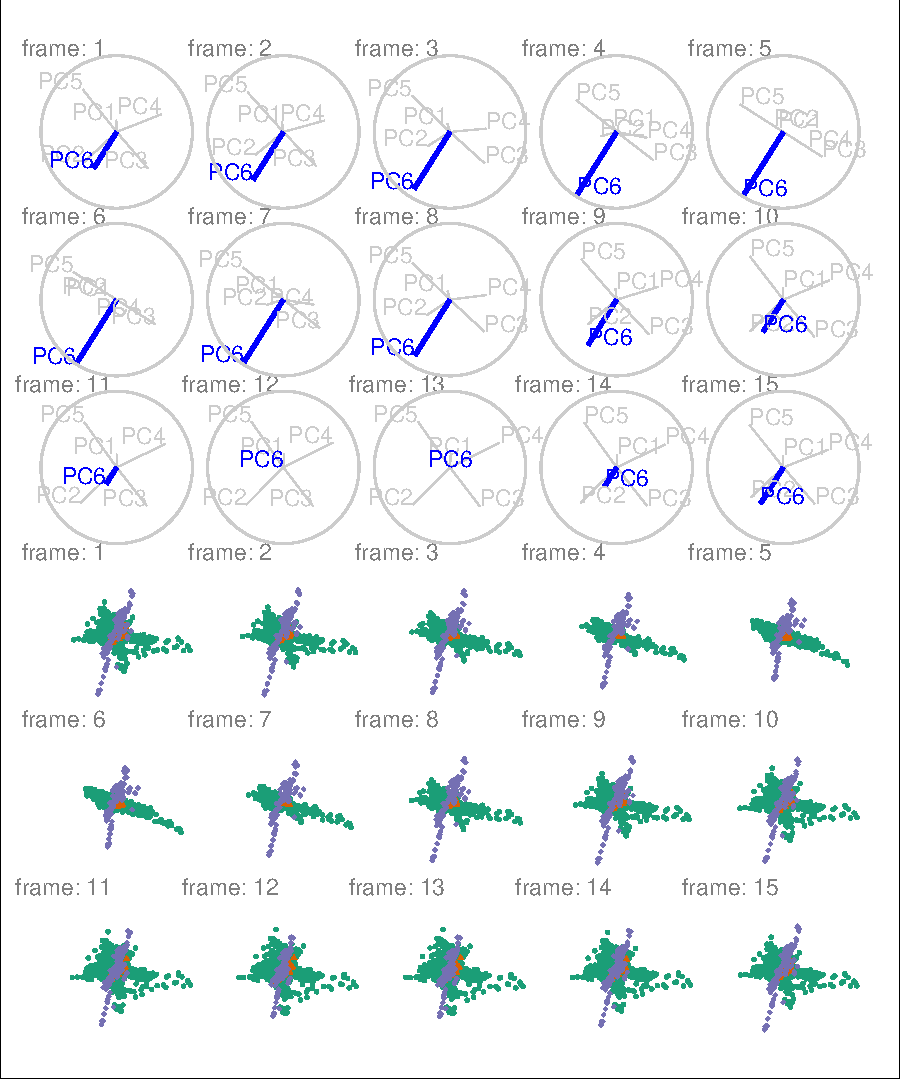
\includegraphics[width=6in,height=7.2in]{spinifex_paper_files/figure-latex/DISclusterGood-1} 

}

\caption[A radial manual tour manipulating the contribution of  PC6 within the DIS cluster]{A radial manual tour manipulating the contribution of  PC6 within the DIS cluster. Points are colored by experiment type: DIS HERA1+2 in green, dimuon SIDIS in purple, and charm SIDIS in orange. The cluster DIS HERA1+2 (green) is distributed in a cross-shaped plane, charm SIDIS (orange) occupies the center space of this cross, with the plane projecting into the field of view when the contribution of PC6 is max. Less evident is the linear dimuon SIDIS (purple) observations approaching the line of view for intermediate values of PC6. A dynamic version can be viewed at https://nspyrison.netlify.com/thesis/discluster\_manualtour\_pc6/.}\label{fig:DISclusterGood}
\end{figure}
\end{Schunk}

\begin{Schunk}
\begin{figure}

{\centering 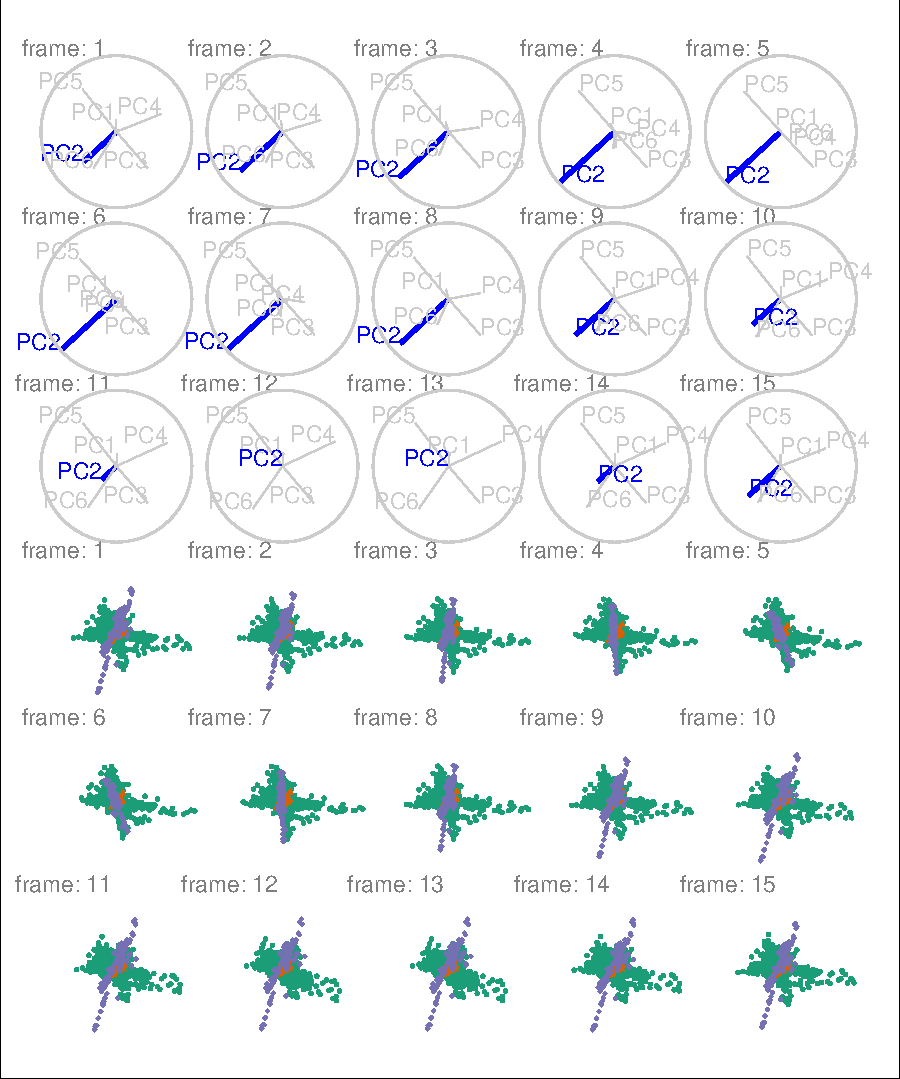
\includegraphics[width=6in,height=7.2in]{spinifex_paper_files/figure-latex/DISclusterBad-1} 

}

\caption[A radial manual tour manipulating the contribution of PC2 within the DIS cluster]{A radial manual tour manipulating the contribution of PC2 within the DIS cluster. Points are colored by experiment type: DIS HERA1+2 in green, dimuon SIDIS in purple, and charm SIDIS in orange. The plane of cross distributed DIS HERA data (green) and a nearly orthogonal jet of dimuon SIDIS (purple) is present. This jet does extend more in the plane of view when the contribution of PC2 is full, giving insight to its orientation. However, less information about the shape of DIS HERA (green) and charm SIDIS (orange) is available. A dynamic version can be viewed at https://nspyrison.netlify.com/thesis/discluster\_manualtour\_pc2/.}\label{fig:DISclusterBad}
\end{figure}
\end{Schunk}

\hypertarget{summary}{%
\subsection{Summary}\label{summary}}

Tours, which are a dynamic linear projection of multivariate data, play
an important role in data visualization; they extend the dimensionality
of visuals while data- and parameter-spaces become ever larger. This
research has modified the algorithm producing manual tours which and has
made this functionality available in package \textbf{spinifex}. The
package adds to \textbf{tourr}, extending the graphics offerings that
can be used to display tours.

Radial manual tours were applied to a dataset across different
experiments of hadronic collisions. The importance of selecting the
correct variable to manipulate is demonstrated by comparing tours of
varying quality. The manual tours convey a better picture of the
structure of the clustering than static linear or non-linear
projections. Giving the full contribution of the manipulation space to
the manip var enables analysts to explore the sensitivity of the
structure with the selected variable. This information can be used by
physicists to identify which experiments are probing which parameter
spaces, which can be indispensable for smarter planning of effort and
funding.

\hypertarget{sec:discussion}{%
\section{Discussion}\label{sec:discussion}}

Future research on the algorithm would include extending it for use in
3D projections. The addition of another dimension theoretically allows
for improved perception. This could explore interactions in immersive
virtual reality or mixed reality, which may further allow for a better
perception of structure and aid in higher-dimensional function
visualization. Functions with many parameters suffer from the same
dimensionality problem as data while their possible values lie on a
plane of values rather than discrete points. Occulation, or the closer
surface blocking further surfaces, will likely be an issue that may be
alleviated by the use of wire mesh, changing opacity, or looking at
sections of the projections (Furnas and Buja
\protect\hyperlink{ref-furnas_prosection_1994}{1994}).

The \textbf{tourr} package provides many other geometric displays with
the \texttt{tourr::display\_*()} family. These geometric options could
be integrated into the \textbf{ggplot2} framework for display on
\textbf{plotly} and \textbf{gganimate}. Additionally, the
\CRANpkg{animation} package Xie et al.
(\protect\hyperlink{ref-xie_animation:_2018}{2018}) could be implemented
for another graphics framework. However, \textbf{animation} builds from
\textbf{base} graphics while \textbf{spinifex} utilizes \textbf{ggplot2}
graphics, a significant paradigm shift.

The Givens rotations and Householder reflections as outlined in Buja et
al. (\protect\hyperlink{ref-buja_computational_2005}{2005}) could also
be added. Currently, Gram-Schmidt is the only form of frame
interpolation used (not used in manual tours). In a Givens rotation, the
\(x\) and \(y\) components (for example \(\theta~= 0,~pi/2\)) of the
in-plane rotation are calculated separately and would be applied
sequentially to produce the radial rotation. Householder reflections
define reflection axes to project points on to the axes and generate
rotations.

Having a script only interaction with tours causes a significant barrier
to entry. To a lesser extent, \textbf{plotly} offers some static
interactions with the contained object, such as tooltips, brushing, and
linking without communicating back to the R console. The development of
a dynamic graphical user interface, perhaps with the use of a
\CRANpkg{shiny} (Chang et al.
\protect\hyperlink{ref-chang_shiny:_2018}{2018}) application, would
mitigate the barrier to entry, allow for more rapid analysis, and offer
an approachable demo tool. The user could easily switch between
variables to control, adjust interpolation step angle, or flag/save
specific frame basis sets.

\hypertarget{acknowledgments}{%
\section{Acknowledgments}\label{acknowledgments}}

This article was created in R (R Core Team
\protect\hyperlink{ref-r_core_team_r:_2018}{2018}), using
\CRANpkg{knitr} (Xie \protect\hyperlink{ref-stodden_knitr:_2014}{2014})
and \CRANpkg{rmarkdown} (Xie, Allaire, and Grolemund
\protect\hyperlink{ref-xie_r_2018}{2018}), with code generating the
examples inline. The source files for this article be found at
\href{https://github.com/nspyrison/spinifex_paper/}{github.com/nspyrison/spinifex\_paper/}.
The source code for the \textbf{spinifex} package can be found at
\href{https://github.com/nspyrison/spinifex/}{github.com/nspyrison/spinifex/}.

\hypertarget{bibliography}{%
\section*{Bibliography}\label{bibliography}}
\addcontentsline{toc}{section}{Bibliography}

\hypertarget{refs}{}
\leavevmode\hypertarget{ref-asimov_grand_1985}{}%
Asimov, Daniel. 1985. ``The Grand Tour: A Tool for Viewing
Multidimensional Data.'' \emph{SIAM Journal on Scientific and
Statistical Computing} 6 (1): 128--43.
\url{https://doi.org/https://doi.org/10.1137/0906011}.

\leavevmode\hypertarget{ref-buja_computational_2005}{}%
Buja, Andreas, Dianne Cook, Daniel Asimov, and Catherine Hurley. 2005.
``Computational Methods for High-Dimensional Rotations in Data
Visualization.'' In \emph{Handbook of Statistics}, 24:391--413.
Elsevier. \url{https://doi.org/10.1016/S0169-7161(04)24014-7}.

\leavevmode\hypertarget{ref-chang_shiny:_2018}{}%
Chang, Winston, Joe Cheng, J. J. Allaire, Yihui Xie, and Jonathan
McPherson. 2018. \emph{Shiny: Web Application Framework for R}.
\url{https://CRAN.R-project.org/package=shiny}.

\leavevmode\hypertarget{ref-cook_manual_1997}{}%
Cook, Dianne, and Andreas Buja. 1997. ``Manual Controls for
High-Dimensional Data Projections.'' \emph{Journal of Computational and
Graphical Statistics} 6 (4): 464--80.
\url{https://doi.org/10.2307/1390747}.

\leavevmode\hypertarget{ref-cook_dynamical_2018}{}%
Cook, Dianne, Ursula Laa, and German Valencia. 2018. ``Dynamical
Projections for the Visualization of PDFSense Data.'' \emph{Eur. Phys.
J. C} 78 (9): 742. \url{https://doi.org/10.1140/epjc/s10052-018-6205-2}.

\leavevmode\hypertarget{ref-furnas_prosection_1994}{}%
Furnas, George W., and Andreas Buja. 1994. ``Prosection Views:
Dimensional Inference Through Sections and Projections.'' \emph{Journal
of Computational and Graphical Statistics} 3 (4): 323--53.
\url{https://doi.org/10.2307/1390897}.

\leavevmode\hypertarget{ref-hurley_analyzing_1990}{}%
Hurley, C., and A. Buja. 1990. ``Analyzing High-Dimensional Data with
Motion Graphics.'' \emph{SIAM Journal on Scientific and Statistical
Computing} 11 (6): 1193--1211. \url{https://doi.org/10.1137/0911068}.

\leavevmode\hypertarget{ref-kirkpatrick_optimization_1983}{}%
Kirkpatrick, Scott, C. Daniel Gelatt, and Mario P. Vecchi. 1983.
``Optimization by Simulated Annealing.'' \emph{Science} 220 (4598):
671--80. \url{https://doi.org/10.1126/science.220.4598.671}.

\leavevmode\hypertarget{ref-lubischew_use_1962}{}%
Lubischew, Alexander A. 1962. ``On the Use of Discriminant Functions in
Taxonomy.'' \emph{Biometrics}, 455--77.
\url{https://doi.org/10.2307/2527894}.

\leavevmode\hypertarget{ref-pedersen_gganimate:_2019}{}%
Pedersen, Thomas Lin, and David Robinson. 2019. \emph{Gganimate: A
Grammar of Animated Graphics}.
\url{http://github.com/thomasp85/gganimate}.

\leavevmode\hypertarget{ref-r_core_team_r:_2018}{}%
R Core Team. 2018. \emph{R: A Language and Environment for Statistical
Computing}. Vienna, Austria: R Foundation for Statistical Computing.
\url{https://www.R-project.org/}.

\leavevmode\hypertarget{ref-sievert_plotly_2018}{}%
Sievert, Carson. 2018. \emph{Plotly for R}.
\url{https://plotly-book.cpsievert.me}.

\leavevmode\hypertarget{ref-wang_mapping_2018}{}%
Wang, Bo-Ting, T. J. Hobbs, Sean Doyle, Jun Gao, Tie-Jiun Hou, Pavel M.
Nadolsky, and Fredrick I. Olness. 2018. ``Mapping the Sensitivity of
Hadronic Experiments to Nucleon Structure.'' \emph{Physical Review D} 98
(9): 094030. \url{https://doi.org/10.1103/PhysRevD.98.094030}.

\leavevmode\hypertarget{ref-wickham_ggplot2:_2016}{}%
Wickham, Hadley. 2016. \emph{Ggplot2: Elegant Graphics for Data
Analysis}. Springer-Verlag New York. \url{http://ggplot2.org}.

\leavevmode\hypertarget{ref-wickham_tourr_2011}{}%
Wickham, Hadley, Dianne Cook, Heike Hofmann, and Andreas Buja. 2011.
``\textbf{Tourr} : An \emph{R} Package for Exploring Multivariate Data
with Projections.'' \emph{Journal of Statistical Software} 40 (2).
\url{https://doi.org/10.18637/jss.v040.i02}.

\leavevmode\hypertarget{ref-stodden_knitr:_2014}{}%
Xie, Yihui. 2014. ``Knitr: A Comprehensive Tool for Reproducible
Research in R.'' In \emph{Implementing Reproducible Computational
Research}, edited by Victoria Stodden, Friedrich Leisch, and Roger D.
Peng. Chapman; Hall/CRC.
\url{http://www.crcpress.com/product/isbn/9781466561595}.

\leavevmode\hypertarget{ref-xie_r_2018}{}%
Xie, Yihui, J. J. Allaire, and Garrett Grolemund. 2018. \emph{R
Markdown: The Definitive Guide}. Boca Raton, Florida: Chapman; Hall/CRC.
\url{https://bookdown.org/yihui/rmarkdown}.

\leavevmode\hypertarget{ref-xie_animation:_2018}{}%
Xie, Yihui, Christian Mueller, Lijia Yu, and Weicheng Zhu. 2018.
\emph{Animation: A Gallery of Animations in Statistics and Utilities to
Create Animations}. \url{https://yihui.name/animation}.

\bibliography{spinifex\_paper.bib}

\address{%
Nicholas Spyrison\\
Monash University\\
Faculty of Information Technology\\
}
\href{mailto:Nicholas.Spyrison@monash.edu}{\nolinkurl{Nicholas.Spyrison@monash.edu}}

\address{%
Dianne Cook\\
Monash University\\
Department of Econometrics and Business Statistics\\
}
\href{mailto:DiCook@monash.edu}{\nolinkurl{DiCook@monash.edu}}

